\documentclass[12pt,notitlepage]{article}
\usepackage[margin=0.75in]{geometry} %1 in margins
\usepackage{graphicx} %For including graphics
\usepackage[labelfont=bf]{caption} %Make float labels bold
%\usepackage{subcaption}
\usepackage{amsmath}

\usepackage[T1]{fontenc}
%\usepackage[utf8]{inputenc}
\usepackage{authblk}

\usepackage[colorlinks, pdfborder={0 0 0}, plainpages=false]{hyperref}
\usepackage{url}

\usepackage{setspace}
%\onehalfspacing % or \doublespacing

\usepackage{times}

%\setlength{\voffset}{-0.5in}
%\setlength{\textheight}{710pt}

\usepackage{wrapfig}

%%%%%%%%%%%%%%%%%%%%%%%%%%%%%%%%%%%%%%%%%%%%%%%%%%%%%%%%%%%%%%%

\begin{document}

\title{Interactive Twitter Data Visualization \\
Word Cloud}

\author[1]{Mehmet Duman} 

\affil[1]{Data Science Graduate Student, University of Massachusetts Dartmouth, Dartmouth, MA 02747, USA}

\date{\today}

\maketitle

\begin{abstract}
The main contribution of this paper is analyzing the data available for Twitter in 2016 USA 
presidential election and trying to express the correlation between social media twitter top subjects before election and the actual result. I used Python multiprocessing system for manipulate tweet dataset, clean the data and create popular use word file. Moreover, this paper is also making assumptions about whether we can guess the results of a future election by observing the past tweets.

\end{abstract}



\newpage

%%%%%%%%%%%%%%%%%%%%%%%%%%%%%%%%%%%%%%%%%%%%%%%%%%%%%%%%%%%%%%%%%%%%%%%%%%%%%%%
\section{Introduction}
%%%%%%%%%%%%%%%%%%%%%%%%%%%%%%%%%%%%%%%%%%%%%%%%%%%%%%%%%%%%%%%%%%%%%%%%%%%%%%%

Data visualization plays an important role in data analysis workflows. It enables data analysts to effectively discover patterns in large datasets through graphical means, and to represent these findings in a meaningful and effective way. 

In this paper by using Python multiprocessing, I aim to analyze active Twitter data and try to achieve following goals:

\begin{enumerate}
\item Get data from twitter network and generate Most Used Word visualization
\item Find historical twitter data for 2016 Presidential Election day 
\item Create Word Cloud to analyze twitter social media for selected filter
\end{enumerate}


I picked Twitter for my paper because it is a very popular social network with many users from different ages. Twitter is an online news and social networking service where users post and read short 140-character messages called "tweets". Registered users can post and read tweets, but those who are unregistered can only read them \cite{Wikipedia:2016}. By 2016, every second, on average, around 6,000 tweets are tweeted on Twitter, which corresponds to over 350,000 tweets sent per minute, 500 million tweets per day and around 200 billion tweets per year \cite{Sayce:2010}. Users share thoughts, links and pictures on Twitter, journalists comment on live events, companies promote products and engage with customers.

For example, on the day of United States Presidential Election 2016, by 10 p.m., 40 million posts had been sent about the election, exceeding the 31 million sent on Election Day 2012 \cite{IsaacEmber:2016}. Although Twitter allows users to post as many tweets as they want, it only allows to get 3,200 of a Users most recent Tweets  (by screen name or user id) \cite{UserTimeline:2016}. 


%%%%%%%%%%%%%%%%%%%%%%%%%%%%%%%%%%%%%%%%%%%%%%%%%%%%%%%%%%%%%%%%%%%%%%%%%%%%%%%
\section{Background}
\label{sec:background}
%%%%%%%%%%%%%%%%%%%%%%%%%%%%%%%%%%%%%%%%%%%%%%%%%%%%%%%%%%%%%%%%%%%%%%%%%%%%%%%

There are some studies that used Twitter, 
\begin{enumerate}
\item Mining Twitter User Profile on Python \cite{Xu:2014} :  
This is an informative slideshare tutorial prepared by PHD student Weiai Xu, and explains how to download Twitter data. It keeps the data in SQLite, and does not do any wordclouds.


\item Analyzing a NHL Playoff Game With Twitter \cite{Forstyh:2014} :
This NHL Playoff Game With Twitter analysis  is written by Python and used Pandas, Python libraries Tweepy, pymongo, vincent and nltk (natural language processing library, for plot text with frequencies). There are some similarities like calculating word frequencies, using stopwords for data cleaning. They generate word versus frequencies plot, but  I believe using wordcloud should be more effective. 


\item Using Python to Grab Twitter User Data \cite{Saxton:2014} :
This work is about using Python Twython library to grab twitter user data. I used Python Tweepy library which is much easier and reliable to get tweets from Twitter Streaming API. This paper does not do any analysis on wordcloud.

\end{enumerate}
	

%%%%%%%%%%%%%%%%%%%%%%%%%%%%%%%%%%%%%%%%%%%%%%%%%%%%%%%%%%%%%%%%%%%%%%%%%%%%%%%
\section{Results}
\label{sec:popul-train-set}
%%%%%%%%%%%%%%%%%%%%%%%%%%%%%%%%%%%%%%%%%%%%%%%%%%%%%%%%%%%%%%%%%%%%%%%%%%%%%%%

In this first part, I am going to explain how I collect the data, by creating different kind of word cloud visualization to analyze dataset. There are different options to collect data from Twitter. I preferred to get tweets by connecting Twitter API network and get real time tweets for my dataset. 

In my project I used following programs;
\begin{itemize}
	\item{Python} : Tweepy library for accessing Twitter API , JSON and Wordcloud library 
	\item JavaScript 
	\item D3.js Visualization
\end{itemize}
	
%-------------------------------------------------------------
\subsection{How to Get Tweets?} 
%-------------------------------------------------------------


	
When I was using python, one of the first libraries I came across was Tweepy, an open source, easy to use python library for accessing the Twitter API. There are three different ways to get access to Twitters enormous amounts of data \cite{Forstyh:2014}. 

\begin{enumerate}
\item First is Twitters Search API which allows you to gather tweets which were made in the past week. You can collect tweets based on user, keywords, locations, its basically the same as when you are searching for tweets on Twitters website except you are limited to how much you can collect and you get raw json type Tweet files. 

\item Second one is Twitter Streaming API. This allows you to compile tweets as they are happening in real time. In order to have access to Twitter data programmatically, we need to create an app that interacts with the Twitter Streaming API. You won't actually use the app for anything, you just need the password and authentication code.The disadvantage of the streaming API is you are not collecting all of the Tweets that are being sent in real time only a sample of ~1\% of the current traffic. 

\item The only way to get the full stream of all tweets being sent that match your criteria is the Twitter Firehose. The only way to get access to the Firehose is to go through a third party such as Datasift or the recently acquired by twitter, GNIP. 
\end{enumerate}



%-------------------------------------------------------------
\subsubsection{Twitter API Access Information} 
%-------------------------------------------------------------

In order to access Twitter Streaming API, we need to get 4 pieces of information from Twitter: API key, API secret, Access token and Access token secret. Then we follow the steps below to get all 4 elements:
\begin{itemize}
	\item Create a twitter account if you do not already have one.
	\item Go to \url{https://apps.twitter.com/} and log in with your twitter credentials.
	\item Click "Create New App"
	\item Fill out the form, agree to the terms, and click "Create your Twitter application"
	\item In the next page, click on "API keys" tab, and copy your "API key" and "API secret".
	\item Scroll down and click "Create my access token", and copy your "Access token" and "Access token secret".
\end{itemize}



%-------------------------------------------------------------
\subsubsection{Connect Twitter Streaming API} 
%-------------------------------------------------------------




I am using a Python library called Tweepy to connect to Twitter Streaming API and
downloading the data. In order to authorize our app to access Twitter on our behalf, we need to use the OAuth interface. The api variable is now our entry point for most of the operations we can perform with Twitter.


\begin{figure}[htb]
	\centering
	\includegraphics[width=0.9\linewidth]{ConnectTwitterStreamingApi.pdf}
	\caption{}
	\label{fig:ConnectTwitterStreamingApi}
\end{figure}


%-------------------------------------------------------------
\subsubsection{Streaming} 
%-------------------------------------------------------------

In order to "keep the connection open", and gather all the upcoming tweets about a particular event, the Streaming API is what we need. We need to extend the StreamListener() to customize the way we process the incoming data. The  Streaming API monitors for tweets and actions in real time and catches them when some event happens. \\

The below script will retrieve each tweet in json file format. I got these tweets text future only and append it as a new line in text file format. Depending on the search term, we can gather tons of tweets within a few minutes. This is especially true for election or live events with a world-wide coverage (World Cups, Super Bowls, Academy Awards, etc) \cite{Bonzanini:2015}.

\begin{figure}[htb]
	\centering
	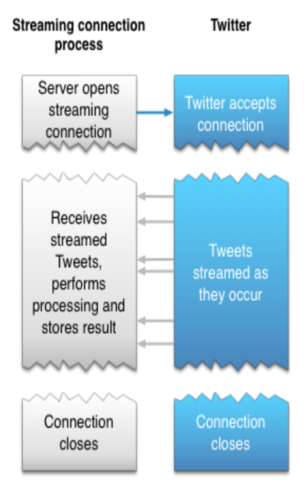
\includegraphics[width=0.2\linewidth]{Streaming_1.pdf}
	\caption{}
	\label{fig:Streaming_1}
\end{figure}


\newpage

\begin{figure}[htb]
%	\centering
	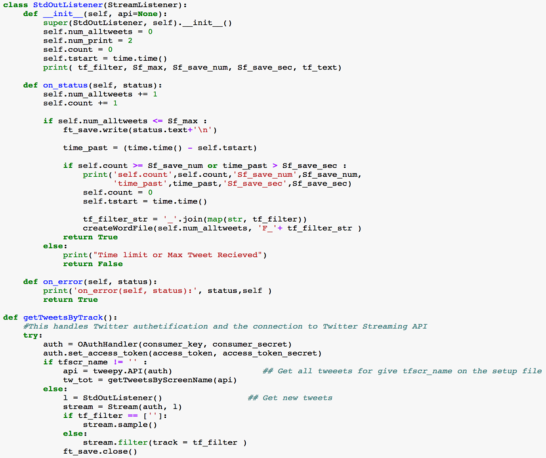
\includegraphics[width=1.2\linewidth]{Streaming_2.pdf}
	\caption{}
	\label{fig:Streaming_2}
\end{figure}




%-------------------------------------------------------------
\subsubsection{Get Tweets for a Specified User} 
%-------------------------------------------------------------


I am using Tweepy library and python to return the tweets of a specified user. According to the Python Twitter Api, they'll allow you to extract a maximum of 3,200 tweets, 200 at a time. To get this 3200 tweets I need to create a loop and each time I could retrieve 200 tweets from user timeline method. This method is different than Twitter API Streaming method. You are getting tweets from specified users timeline and there is no time limits for this last 3200 tweets.  
\\





%-------------------------------------------------------------
\subsection{Tweet Sample} 
%-------------------------------------------------------------

Tweet text is limited by 140 character, but single tweet is around 2000 character.

\begin{figure}[htb]
	\centering
	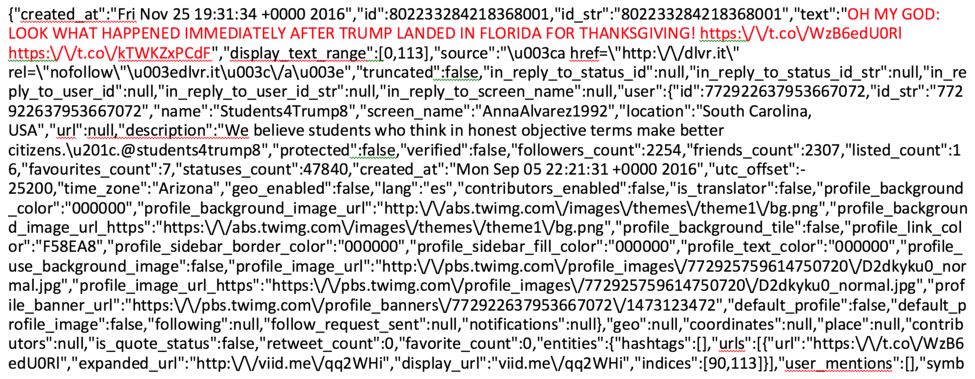
\includegraphics[width=1\linewidth]{TweetSample.pdf}
	\caption{}
	\label{fig:TweetSample}
\end{figure}




%-------------------------------------------------------------
\subsection{Using Python Multiprocessing to Read and Process Tweets} 
%-------------------------------------------------------------

\begin{wrapfigure}{r}{0.65\linewidth}
	\vspace{-20pt}
	\centering
	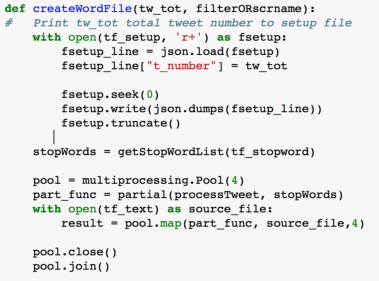
\includegraphics[width=1\linewidth]{PyMultiprocessing_1.pdf}
	\caption{}
	\label{fig:PyMultiprocessing_1}
\end{wrapfigure}



Python multiprocessing pool: It is a process pool object which controls a pool of worker processes to which jobs can be submitted. \\
Python map (func, iterable, [chunksize]): This object will lock the main program until all a process is finished, which is quite useful if we want to obtain result in a particular order for certain applications. \\


While I am getting tweets from the Twitter Streaming API, I am writing every tweets text info in a "tweet text file". If my tweet counter exceed the number from TwitterSetup.txt "tweet number", I am processing "tweet text file" to generate popular used word files (You can see the python code above  Figure:\ref{fig:Streaming_2}) and wordcloud image. During this process I am using python Multiprocessing to speed up.  This generating file process is keep repeating whenever tweet counter exceeds the "tweet number" and generates wordcloud images.\\

\begin{figure}[htb]
	\centering
	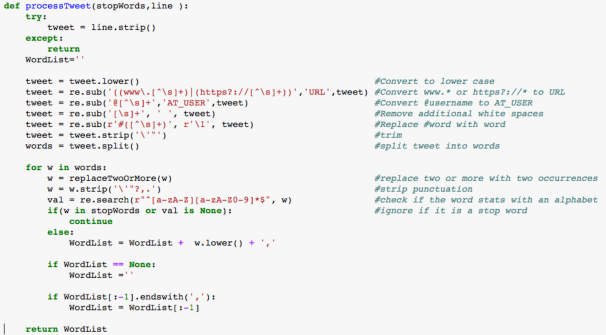
\includegraphics[width=1.2\linewidth]{PyMultiprocessing_2.pdf}
	\caption{}
	\label{fig:PyMultiprocessing_2}
\end{figure}



%-------------------------------------------------------------
\subsection{Creating Word Cloud by Python WordCloud Library} 
%-------------------------------------------------------------


A worldcloud is a collage of words and those words that are bigger in size have a high frequency. Python wordcloud library is very special and easy to use. This library module will automatically clean a text such as split the sentence and delete some stop-words and generate the wordcloud.

\begin{figure}[htb]
	\centering
	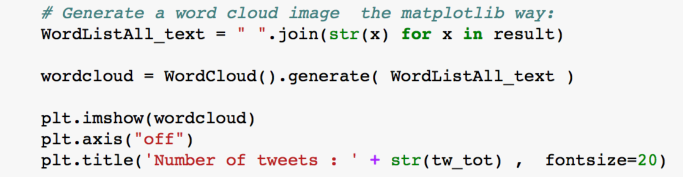
\includegraphics[width=0.9\linewidth]{PyWordCloud_1.pdf}
	\caption{}
	\label{fig:PyWordCloud_1}
\end{figure}


After I generate "result" list variable (from Figure:\ref{fig:PyMultiprocessing_1})  by using Python Multiprocessing, I just use Python wordcloud library to generate the word cloud and save it to file.  Creating wordcloud process is like, I am taking a picture of current tweets status and copying current tweets file to another file. After I generate my word cloud, I keep continue to retrieve tweets from Twitter and append to the existing file. 

By generating wordcloud image over and over again in certain time or by certain tweet number (this control number is defined in TwitterSetup.txt), I can follow the changes on the word clouds in time period and keep it in record.


%-------------------------------------------------------------
\subsection{Creating animated Word Cloud by D3.javascript} 
%-------------------------------------------------------------

Python wordcloud library is a great tool, but I like to show and update the changes on the screen in real time. This is not possible by Python wordcloud. Therefore, I used animated d3 word cloud example \cite{Whitfield:2016} with prepared by D3.javascript  and implemented into my project. By generating this d3.javascript application, I am able to generate animated word cloud, bring focus on the important changes by transition animation and get updates for new popular words interactively.
\\

For this job, I need to calculate/define each popular words weight manually. I count the words frequencies and created popular top 30 words from text file. When I am creating this file, I used below mathematical logic to define words weight from popular words frequencies.\\
\\

\begin{wrapfigure}{r}{0.6\textwidth}
	\vspace{-42pt}
	\centering
	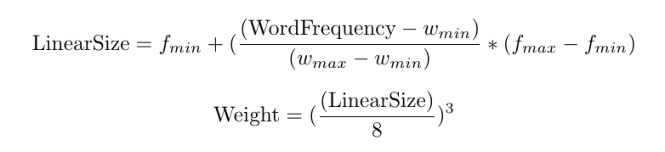
\includegraphics[width=0.5\textwidth]{D3jsWordCloud_1.pdf}
	\caption{}
	\label{fig:D3jsWordCloud_1}
\end{wrapfigure}


$w_{min}$ : minimum word frequency  \

$w_{max}$ : maximum word frequency \

$f_{min}$ : minimum font size \

$f_{max}$ : maximum font size \

\begin{figure}[htb]
	\centering
	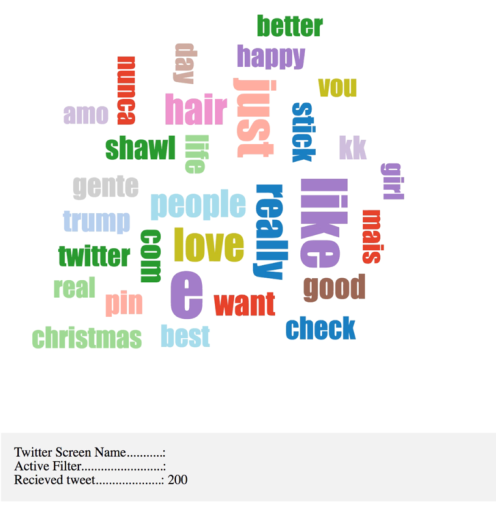
\includegraphics[width=0.4\linewidth]{D3jsWordCloud_4.pdf}
	\caption{Sample for animated wordcloud}
	\label{fig:D3jsWordCloud_4}
\end{figure}

\
\\
I created word clouds by Python wordcloud library and D3.js. Each visualization has different kind of advantages. Some of the D3.js wordcloud visualization advantages are, user friendly, the transition can be followed, and new word updates or subtract in real time. You have the all control on word font sizes and styles. Everything is happening interactively. Some of the Python matplotlib wordcloud library advantages are, easy to generate plots, could be save to a file in periodically to keep record of word clouds. Both visualizations helped me to achieve different kind of goals.




%-------------------------------------------------------------
\subsection{ Wordcloud Analyst} 
%-------------------------------------------------------------

After analyzing my data, I generated many graphs. However, I found a few of them useful for my analysis. Below I have explained them one by one:\



\begin{figure}[htb]
	\centering
	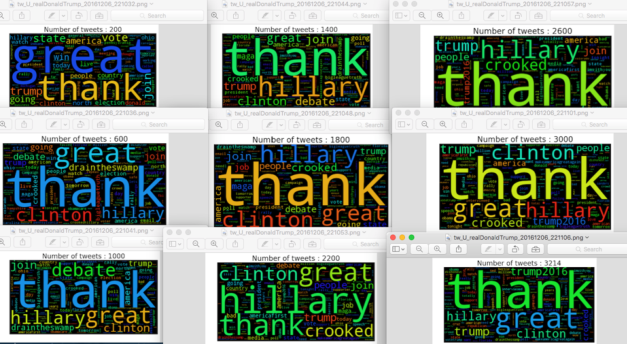
\includegraphics[width=0.79\linewidth]{WordCloudAnalystGana_10.pdf}
	\caption{User @realDonaldTrump}
	\label{fig:WordCloudAnalystGana_10}
\end{figure}

Donald Trump has 34.1K total tweets on his record and Figure:\ref{fig:WordCloudAnalystGana_10} shows his last 3200 tweets before 12/06/2016. As wee see word 'Hillary' shows up after 1000 tweets, and it is the most used one by 2,200 tweets. After 2,600 tweets it shows up in smaller fonts, means user @realDonaldTrump used word 'Hillary' less frequently.



\begin{figure}[htb]
	\centering
	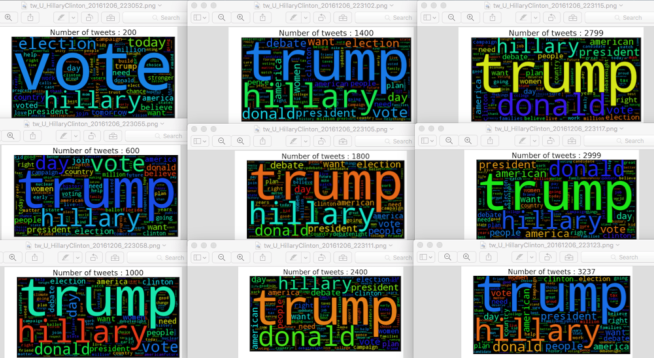
\includegraphics[width=0.79\linewidth]{WordCloudAnalystGana_20.pdf}
	\caption{User @HillaryClinton}
	\label{fig:WordCloudAnalystGana_20}
\end{figure}

Hillary Clinton has 9.8K total tweets on his record and Figure:\ref{fig:WordCloudAnalystGana_20} shows her last 3200 tweets before 12/6/2016. As we see, word 'Donald' shows up after 1,000 tweets and it is popular after 2,400 tweets then by 3,200 tweets its frequency drops. 

\newpage


Filter "Ghana", There where general election at December 7, 2016

\begin{figure}[htb]
	\centering
	\begin{minipage}[b]{0.43\textwidth}
		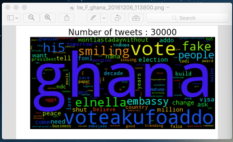
\includegraphics[width=\textwidth]{WordCloudAnalystGana_1.pdf}
		\caption{Dec 6, 8:25am-4:38pm}
		\label{fig:WordCloudAnalystGana_1}
	\end{minipage}
	%	\hfill
	\begin{minipage}[b]{0.4\textwidth}
		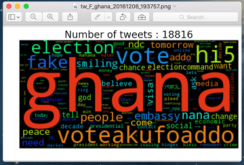
\includegraphics[width=\textwidth]{WordCloudAnalystGana_2.pdf}
		\caption{Dec 6, 5:22pm-12:37am}
		\label{fig:WordCloudAnalystGana_2}
	\end{minipage}
\end{figure}


\begin{figure}[htb]
	\centering
	\begin{minipage}[b]{0.4\textwidth}
		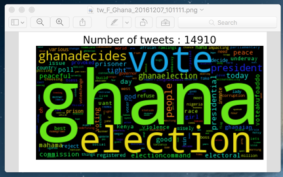
\includegraphics[width=\textwidth]{WordCloudAnalystGana_3.pdf}
		\caption{Dec 7, 10:40am-3:11pm}
		\label{fig:WordCloudAnalystGana_3}
	\end{minipage}
	%	\hfill
	\begin{minipage}[b]{0.15\textwidth}
		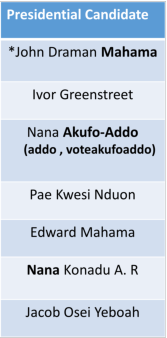
\includegraphics[width=\textwidth]{WordCloudAnalystGana_4.pdf}
		\caption{}
		\label{fig:WordCloudAnalystGana_4}
	\end{minipage}
\end{figure}





These figures show how people's tweets wary before and on the election day. As you see from the Figures, Nana Akufo-Addo (voteakufoaddo) was one of the most tweeted one between candidates, and he won the election.


















%-------------------------------------------------------------
\section{Conclusion} 
%-------------------------------------------------------------

In this paper my aim was to reach my goals, and I could be able to do so. For example, I aimed to get data from twitter and generate the most used word visualization. I was able to get real time new tweets and most recent 3200 tweets for selected users and created wordclouds. 

Secondly, I wanted to find historical twitter data for 2016 Presidential Election day. However, twitter has one-week restriction for old tweets, but if you have tweet ID's you can retrieve older tweets also. 2016 Election day there was more than 40 million tweets. I found tweet ID's for 20 Million tweets for this day, but it was too slow process to retrieve each tweet by their tweet id one by one. 

Next, I wanted to create Word Cloud to analyze twitter social media for selected filter. I was able to do that in many different ways.

During my studies I came across with some difficulties. I tried to use Python Multithreading, but it is so complex. It needs improvement, I wasn't able use it to process tweets. However, I used Python Multiprocessing and it increased the performance of processing tweets significantly. 

If I compare Python and C, I could easily say C OpenMP and C MPI are more powerful, but Python program is really easy to write code and find libraries to use for all kind of needs.
Like Tweepy, it is a great open-source library to access to the Twitter API, heavily relies on it and has great Streaming API support. 

To conclude, my study only shows that it is possible to find out what social media talks about a subject by just using a specific filter, and this can open many doors. With so many users around the globe, Twitter is a very good source for political and social studies, as well as advertisement and marketing studies. If we could be able to use the current and historical data and show the results visually, we can get impromptu results for many major events, and may predict the actual results. Therefore, I believe using Twitter data has a promising future.






%\section*{References}

\bibliographystyle{unsrt}
\bibliography{References}


\end{document}
